\chapter{Resultados y discusión}
\label{resultados}


El principal objetivo de este proyecto una aplicación móvil radio faro que
 funcione como cliente, emitiendo la posición GPS del dispositivo en
 determinadas condiciones, y como monitor para que pueda ser
 localizada la señal del dispositivo que solicita ayuda.

El resultado de este proyecto es una aplicación que intenta cumplir 
con los requisitos planteados y creo que lo hemos conseguido, aunque
 la localización no sea todo lo fiable que nos gustaría hemos conseguido 
un producto que puede ser de utilidad para ayudar a las personas
 en apuros y que puede servir en un futuro como base para implementar
 la arquitectura PEMEA(Pan European Mobile Emergency App)~\cite{PEMEA} y aplicar la misma a un entorno
 marítimo, incluso usar el backend de la aplicación para realizar estudios
 sobre los incidentes reportados para sacar estadísticas y determinar
 puntos negros de nuestro litoral.

A continuación vamos a comentar en que consiste la arquitectura PEMEA
 y a explicar el principal punto de discusión del proyecto, que es el cálculo
 de la velocidad a la que consideramos que un cuerpo se encuentra a la
 deriva en el mar.

\section{Arquitectura PEMEA}

El proyecto PEMEA (Pan-European Mobile Emergency Apps) es una
 inciativa de la unión europea para unificar en una aplicación, la conexión 
con todos los centros de emergencia 112.

El objetivo de este proyecto es proporcionar una arquitectura que permita
 acceder a los servicios de emergencia en cualquier lugar de Europa y un 
endpoing para poder dar acceso a información ampliada del usuario, como
 por ejemplo, a su geolocalización.

El proyecto aún no esta terminado, actualmente esta en fase de pruebas.
 El inicio de la fase 2 esta planificado a principios de Septiembre 2019.

En la siguiente imagen vemos como funciona esta arquitectura.

\begin{figure}[h]
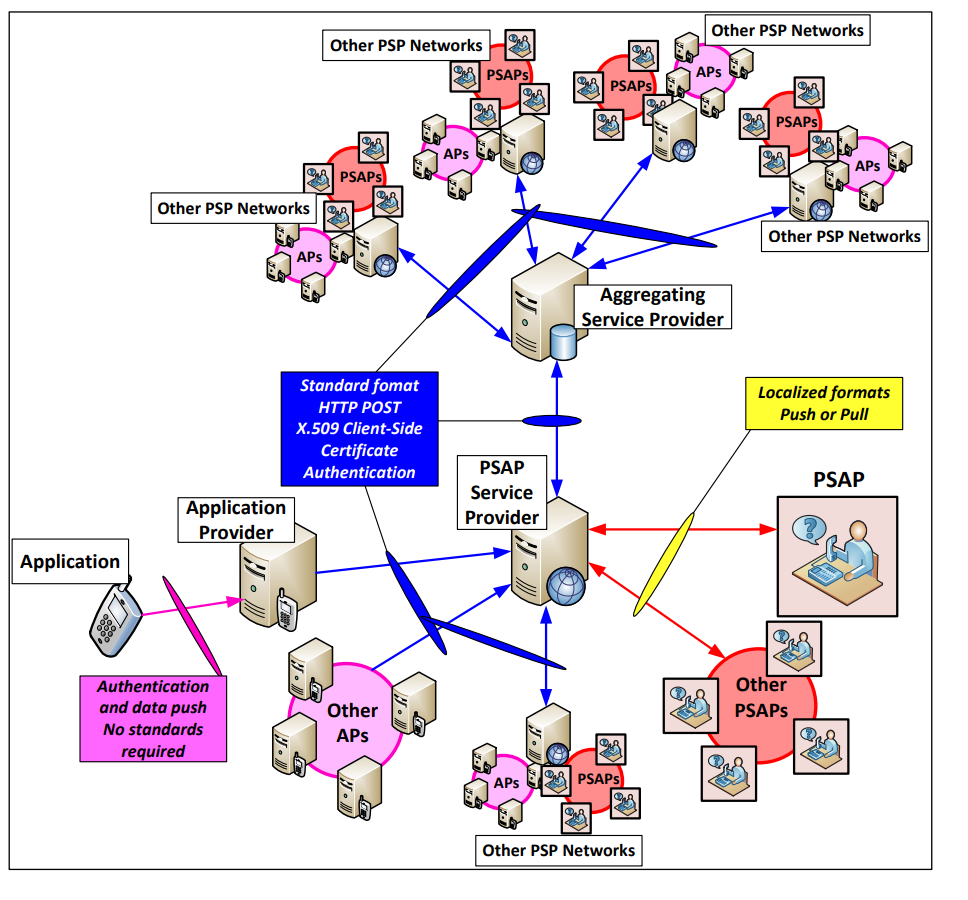
\includegraphics[scale=0.5]{pemea_arq.png} 
\floatfoot{Figura 9. Arquitectura PEMEA completa.}
\end{figure}

\footnote{Fuente: PEMEA~\cite{PEMEA}.}
\section{Pronosticar la deriva de objetos en el océano}

El movimiento de un objeto a la deriva en la superficie del mar es uno 
de los temas de discusión fundamentales de este proyecto. Este
 movimiento es el resultado de varias fuerzas que actúan sobre la superficie:

\begin{enumerate}
\item Corrientes marinas.
\item Viento.
\item Oleaje.
\end{enumerate}


También influye el centro de gravedad del objeto y su forma.

Tenemos dos cuestiones importantes que definir, la dirección 
y la velocidad del objeto a la deriva.

\subsection{Velocidad del objeto}

Después de leer varios estudios y artículos, he llegado a la
 conclusión, que la fórmula para calcular la velocidad de un objeto 
flotando a la deriva, es directamente proporcional a la velocidad
del viento y condicionado por un factor que se calcula empíricamente
 o con modelos muy complejos de mecánica de fluidos que no 
tenemos a nuestra disposición, así que vamos a simplificar.

Utilizaremos la siguiente fórmula.
\[\
   x \times \alpha + A \\  
\]

Donde:
\begin{enumerate}
\item $x$ es la velocidad del viento, en m/s.
\item $alpha$ es el coeficiente con valor 0.70.
\item $A$ es la constante de error, que calculamos como un 20\% del valor de $x$.
\end{enumerate}

Fuente: Formulation of Leeway-Drift Velocities for Sea-Surface
Drifting-Objects Based on a Wind-Wave Flume Experiment~\cite{VDERIVA}.



\subsection{Dirección del objeto}


Otro de los puntos más importantes es la dirección de movimiento del 
objeto a la deriva, comúnmente se piensa que es la misma que la del viento,
 pero hay que tener en cuenta la componente cruzada del viento principal, a
 la hora de calcular esta dirección, podemos ver en la siguiente imagen como 
se compone el vector de movimiento del objeto a la deriva.


\begin{figure}[h]
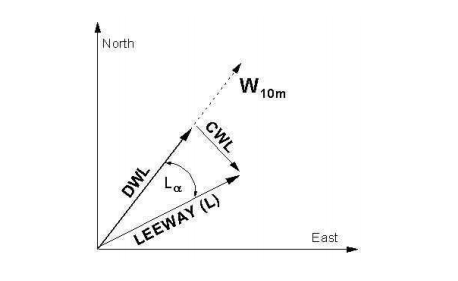
\includegraphics[scale=0.5]{relacion_viento.png} 
\caption{Relacion entre el vector del objeto a la deriva (L), 
el vector del viento (DWL) y el vector del viento cruzado (CWL). L indica el ángulo de deriva. }
\end{figure}


Para solventar en nuestro algoritmo el problema del viento cruzado, vamos a añadir un margen de 
error del treinta por ciento a la hora de calcular la dirección de deriva. 

Fuente: Ocean weather forecasting: An integrated view of oceanography~\cite{DDERIVA}.